\documentclass[12pt, oneside]{article}   	                 		
\usepackage{graphicx}
\usepackage{epstopdf}
\usepackage{cite}
\usepackage{setspace}
\usepackage{mathtools}
\usepackage{amsmath}
\usepackage{amssymb}
\usepackage{caption}
\usepackage{subcaption}
\usepackage{tabularx}
\usepackage{fullpage}  
\usepackage{enumerate}
\usepackage{enumitem}
\setlist{nolistsep}
\usepackage{url} 
\usepackage{multicol}
\usepackage{appendix}
\usepackage[section]{placeins}
\usepackage{morefloats}
\usepackage{topcapt}
\graphicspath{{/home/wwwennie/wwwennie@gmail.com/UT-Austin/teaching/Elective-Computational-Methods-MatSci/projects/3-lattice-sums-defects/figs/}}

\title{PSet 3: Lattice Sums, Part 2}
\author{Solutions}
\date{}


\begin{document}
\maketitle

Attached is the following code that was used in this problem set
\vspace{5mm}
 \begin{enumerate}
   \item make\textunderscore latt.py   $\rightarrow$ generating FCC and BCC lattices
   \item lat\textunderscore sum.py   $\rightarrow$ lattice sum routines with Lennard-Jones potential
   \item PS3-*.py     $\rightarrow$ code for generating plots and gathering information, filled with comments on the logic
 \end{enumerate}
 \vspace{5mm}

%--------------------------------------------------------------------------------%
\section{Exercise 1: Vacancy formation in FCC Cu}

We calculate the formation energy of a Cu vacancy in FCC Cu. We choose a cutoff radius slightly greater than the distance of the third nearest neighbor (in FCC, $a_0 \sqrt{(\frac{1}{2})^2+(\frac{3}{2})^2}$) to have an integer number of repeated unit cells. The Lennard-Jones potential is used with parameters $\epsilon = 0.3429 eV, \sigma = 2.553  \AA$. 

The formation energy of a vacancy may be found as 

\begin{equation}
   \Delta U = E_{vac} - \frac{n-1}{n} E_{bulk}
\end{equation}

\noindent where $E_{vac}$ is the energy of the system with a vacancy of (n-1) atoms and $E_{bulk}$ is the energy of bulk of \textit{n} atoms. 

In order to properly simulate the cell, we first find the optimal lattice parameter. As illustrated in Figure \ref{fig:fcccu}, the equilibrium lattice constant for the chosen values of $\epsilon$ and $\sigma$ is about 3.53  \AA, a 2.3\% difference smaller than the experimental value.

\begin{figure}[htbp]
   \centering
   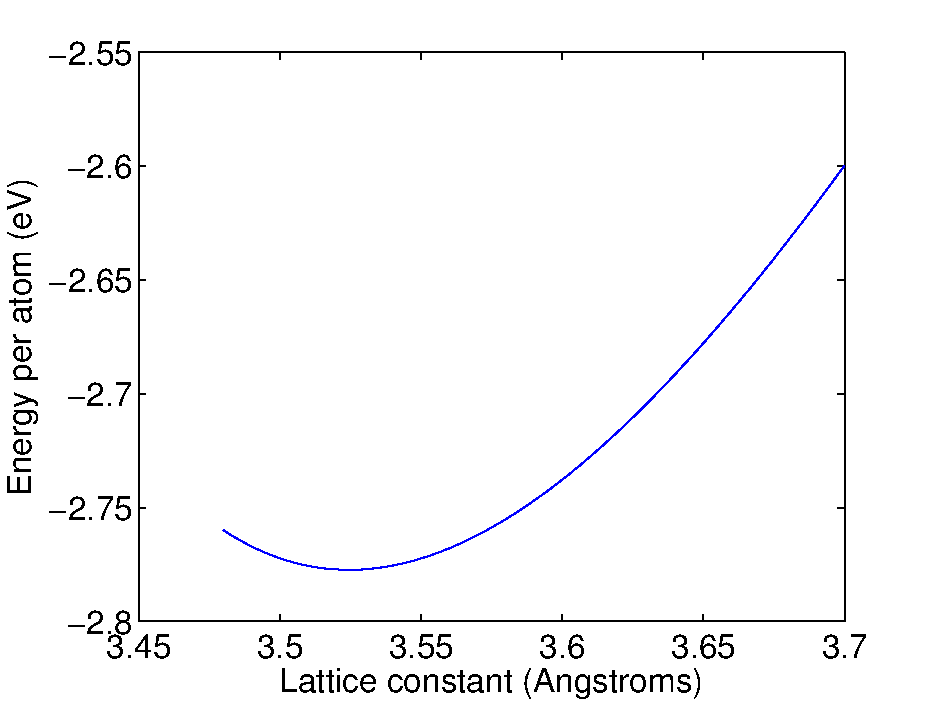
\includegraphics[width=0.8\textwidth]{fcccu} % requires the graphicx package
   \caption{Energy per atom as a function of lattice constant of FCC Cu using Lennard-Jone potential with $\epsilon = 0.3429 eV, \sigma = 2.553  \AA$ }
   \label{fig:fcccu}
\end{figure} 

Using these parameters, we find

\begin{verbatim}
===================
Bulk energy (eV/atom): -2.7767905 for 256 atom cell
Minimum Lattice Energy: -2.777358
Minimum Lattice Energy Lattice constant (Ang): 3.5249999
----------------------------
Vacancy Lattice Energy (eV/atom): -2.76590115 for 255 atom cell
Vacancy formation energy (eV): 2.7767905
===================
\end{verbatim}

The experimental value of the vacancy formation of copper has been measured to range between 0.7 and 1.3 eV (see References). 
For the unrelaxed Cu vacancy simulated with the Lennard-Jones potential, this is an overestimate of nearly four times as large at worst and twice at best.
Sources of discrepancies include primarily not allowing the structure to not relax its internal coordinates around the vacancy, but also having a sufficiently large enough cutoff to capture relevant interactions, L-J potential parameters that accurately represent Cu, and the fact that the L-J potential has limited accuracy in its ability to deal with metals. The last reason is particularly salient as it is known that pair potentials, such as the L-J potential, cannot accurately capture even bulk properties of metals, let alone defect structures (as discussed in Section 5.5.1 of LeSar). 

%--------------------------------------------------------------------------------%
\section{Exercise 7: Relaxation around vacancy in FCC Cu}

To more accurately find the formation energy of the copper vacancy, we relax the coordinate positions of atoms in the nearest shell of neighbors to the vacancy. 

Relaxation involves varying the positions of the atoms. There are several steps that the submitted code goes through in order to accomplish. Due to the spherical-like symmetry of the 12 nearest neighbors that surround the vacancy, we predict that the atoms relax symmetrically about the defect. This effectively means moving each nearest neighbor an equal displacement radially away from the vacancy. For this reason, we choose to implement the displacement of atoms for relaxation in spherical coordinates.

Several subtleties arise from this choice of implementation. 
\vspace{5mm}
 \begin{enumerate}
   \item Because we use the minimum image convention, it is important to make the cutoff distance $r_c$ slightly larger to accommodate relaxation of the atoms.
   \item We choose a specific atom as the vacancy site before any other operations are performed; in order to easily capture this, we choose the atom closest to the center of the simulation cell, and take this coordinate as effectively our new origin. 
   \item In order to displace the atoms an equal amount radially, we use spherical coordinates; this requires converting to and from spherical coordinates back into cartesian coordinates so that it is compatible with latsum5.m
   \item Additionally, the displacement of nearest neighbors is translated to the original origin of the simulation cell for convenience of the math
   \item Converting to and from spherical coordinates results in duplicate coordinates that require an inversion through the original origin
\end{enumerate}
\vspace{5mm}

With relaxation we find 

\begin{verbatim}
Bulk Lattice Energy (eV/atom): -2.776790 for 4 cell
Vacancy Lattice Energy (eV/atom): -2.765901 for 0.0000 disp
Vacancy formation energy (eV): 2.776790 for 0.000 disp 
-------------------------------
Min Formation energy (eV): 2.758171
Vacancy Relax E_min displacement (eV): -0.005102
Vacancy Relax E_min (eV): -705.323414 for system and -2.765974 per atom
Vacancy Energy changed by (eV): -0.018619
===============================

\end{verbatim}

\begin{figure}[htbp]
   \centering
   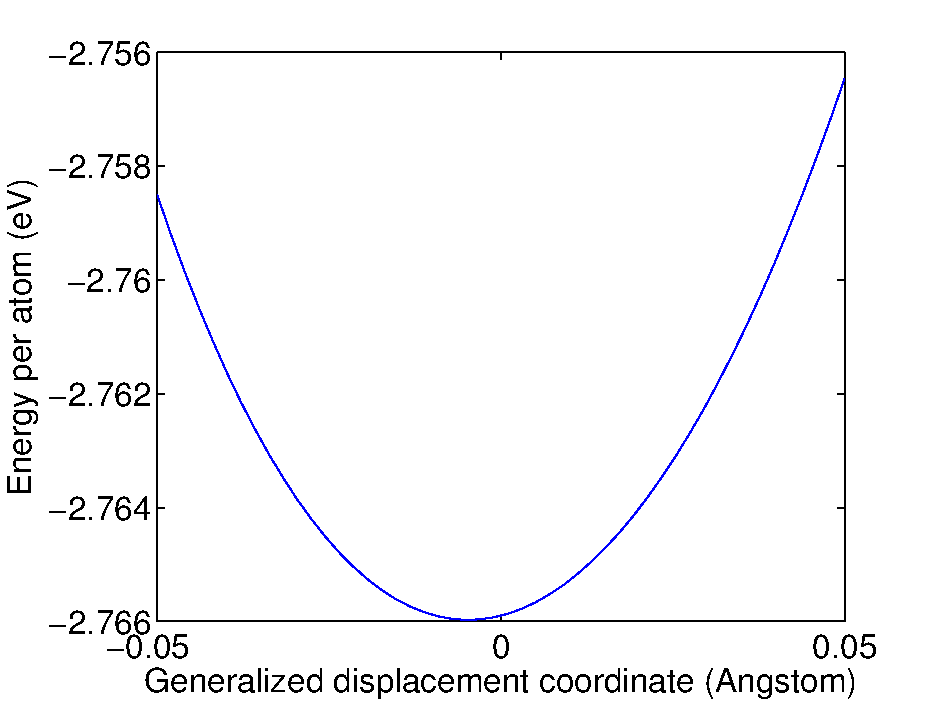
\includegraphics[width=0.8\textwidth]{cuvacrel} % requires the graphicx package
   \caption{Energy per atom as a function of uniformly displacing the nearest neighbors of the vacancy in FCC Cu using L-J potential; the generalized displacement coordinate is the magnitude of change in relative coordinates.}
   \label{fig:cuvacrel}
\end{figure}

This is illustrated in Figure \ref{fig:cuvacrel} which shows the effect on energy per atom in the vacancy structure for contraction (i.e., negative values) and expansion (i.e., positive values) of the nearest neighbor shell around the vacancy. As seen both Figure \ref{fig:cuvacrel} and the above results, relaxation of this method results in the the nearest neighbor shell moving towards the vacancy by about 0.018 \AA  ($ \approx 0.005102 \cdot 3.533 \AA $)

%--------------------------------------------------------------------------------%
\section{Exercise 8: Non-cubic lattices}

We extend our analysis to non-cubic lattices by decreasing the symmetry of the cubic structures tested so far. We keep the angles all $90^o$ for simplicity. In order to compare cubic to non-cubic structures, we keep the same volume and allow the lattice parameters to vary. Figure \ref{fig:noncubic} shows a plot of varying the \textit{b} lattice parameter and the resulting energy per atom.

\begin{figure}[htbp]
   \centering
   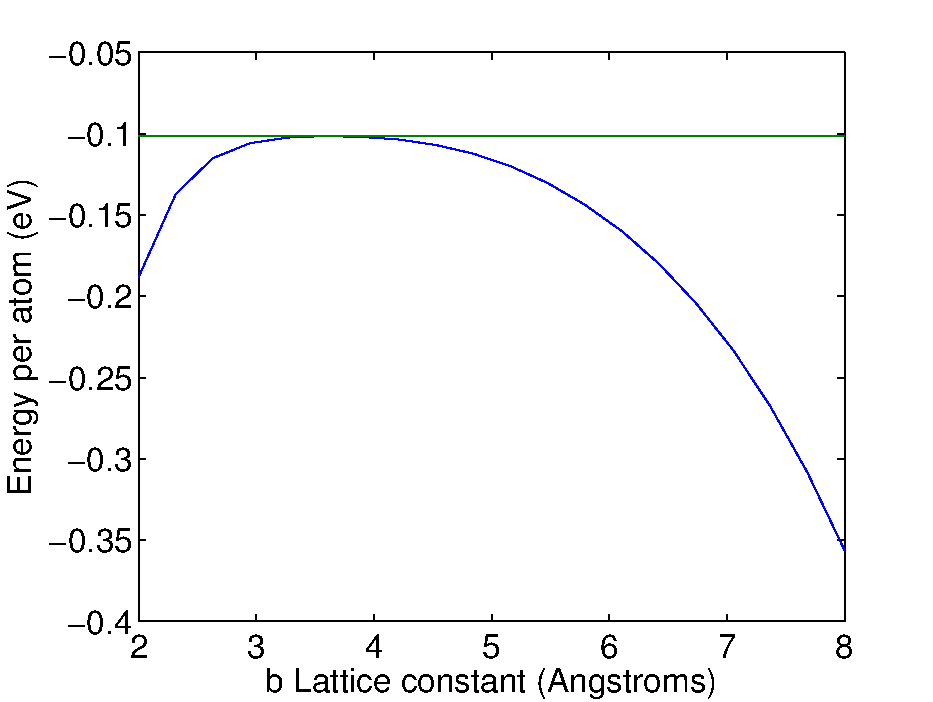
\includegraphics[width=0.8\textwidth]{noncubic} % requires the graphicx package
   \caption{Energy per atom as a function of varying the \textit{b} lattice constant (blue) in comparison to the cubic structure (green), with constant volume; $\epsilon = \sigma = 1$ in L-J potential}
   \label{fig:noncubic}
\end{figure}

 As seen in Figure \ref{fig:noncubic}, allowing asymmetries in the system results in a lower energy per atom.

%--------------------------------------------------------------------------------%
\section{Exercise 9: Bain Transition}

Non-cubic lattices are also relevant to the Bain Transition, which involves the transformation between the \textit{bcc} and \textit{fcc} lattice. The \textit{bcc} structure can be described using the face centered tetragonal (\textit{fct}) structure and has equivalent relative atomic positions to the \textit{fcc} structure. When $a = b = \sqrt{2}c$, the \textit{fct} structure is equivalent to the \textit{bcc} structure for the same volume per atom and cutoff energy. 

From the equilibrium lattice constant of \textit{bcc} found in Pset 2, we can determine the lattice constants to use for \textit{fct}. 

\begin{equation}
 vol_{fct} = a_{fct}^2 c = \frac{a_{fct}^3}{\sqrt{2}}
\end{equation}

\begin{equation}
 vol_{fct/atom} = \frac{a_{fct}^3}{\sqrt{2}} \frac{1}{4}
\end{equation}

\begin{equation}
  vol_{bcc/atom} = a_{bcc}^3 \frac{1}{2}
\end{equation}

\begin{equation}
  \therefore a_{fct}^3 = 2\sqrt{2} a_{bcc}^3
\end{equation}

Using the same volume per atom and energy cutoff indeed result in the same energy, as illustrated in the output below.

\begin{verbatim}
 % ncells = 5
 % BCC Energy: -7.948672 for 5 cell 
 % BCC vol/atom: 0.941826 
 % FCT Energy: -7.948672 for 5 cell 
 % FCT vol/atom: 0.941826 
 % ----------------------------
 
 % ncells = 3
 % BCC Energy: -6.792686 for 3 cell 
 % BCC vol/atom: 0.941826 
 % FCT Energy: -6.792686 for 3 cell 
 % FCT vol/atom: 0.941826 
 % ----------------------------
\end{verbatim}

\section{References}

\noindent C.J. Meechan and R.R. Eggleston. Formation energies of vacancies in gold and copper. \textit{Acta Metallurgica.} \textbf{2} (1954) 680-683.

\hfill

\noindent P. Jongenburger. Energy of formation vacancies in Copper and Gold. \textit{Phys. Rev.} \textbf{106} (1957) 66.

\hfill

\noindent W. Triftsh{\"a}user and J.D. McGervey. Monovacancy formation energy in copper, silver, and gold by positron annihilation. \textit{App. Phys.} \textbf{6} (1975) 177.

\end{document}